% Generated by scripts/rerun/make_figures.py - do not edit by hand.
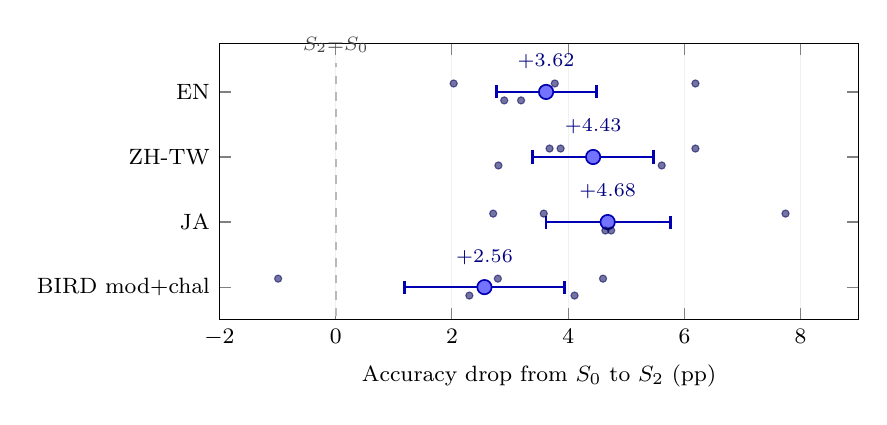
\begin{tikzpicture}
\begin{axis}[
    width=0.8\linewidth, height=0.42\linewidth,
    xmin=-2, xmax=9,
    xlabel={\footnotesize Accuracy drop from $S_0$ to $S_2$ (pp)},
    ytick={1,2,3,4}, yticklabels={BIRD mod+chal, JA, ZH-TW, EN},
    ymin=0.5, ymax=4.75, xtick={-2,0,2,4,6,8},
    tick label style={font=\footnotesize}, label style={font=\footnotesize},
    axis line style={-, line width=0.4pt}, xmajorgrids, grid style={gray!12, line width=0.4pt}, clip=false,
    tick style={line width=0.4pt},
]
\draw[dashed, gray!55, line width=0.6pt] (axis cs:0,0.55) -- (axis cs:0,4.45);
\node[font=\scriptsize, gray!55!black, anchor=south] at (axis cs:0,4.45) {$S_2{=}S_0$};
\addplot[only marks, mark=*, mark size=1.3pt, color=blue!35!black,
         mark options={fill=blue!35!black, fill opacity=0.55, draw opacity=0.55}]
  coordinates {(-0.99,1.13) (4.11,0.87) (4.60,1.13) (2.30,0.87) (2.79,1.13) (2.71,2.13) (4.64,1.87) (3.58,2.13) (4.74,1.87) (7.74,2.13) (3.87,3.13) (2.80,2.87) (3.68,3.13) (5.61,2.87) (6.19,3.13) (3.77,4.13) (2.90,3.87) (2.03,4.13) (3.19,3.87) (6.19,4.13)};
\draw[blue!70!black, line width=1pt] (axis cs:1.18,1)--(axis cs:3.94,1);
\draw[blue!70!black, line width=1pt] (axis cs:1.18,0.9)--(axis cs:1.18,1.1);
\draw[blue!70!black, line width=1pt] (axis cs:3.94,0.9)--(axis cs:3.94,1.1);
\filldraw[blue!55, draw=blue!70!black, line width=0.6pt] (axis cs:2.56,1) circle (2.6pt);
\node[font=\scriptsize, blue!50!black, anchor=south] at (axis cs:2.56,1.2) {$+2.56$};
\draw[blue!70!black, line width=1pt] (axis cs:3.62,2)--(axis cs:5.76,2);
\draw[blue!70!black, line width=1pt] (axis cs:3.62,1.9)--(axis cs:3.62,2.1);
\draw[blue!70!black, line width=1pt] (axis cs:5.76,1.9)--(axis cs:5.76,2.1);
\filldraw[blue!55, draw=blue!70!black, line width=0.6pt] (axis cs:4.68,2) circle (2.6pt);
\node[font=\scriptsize, blue!50!black, anchor=south] at (axis cs:4.68,2.2) {$+4.68$};
\draw[blue!70!black, line width=1pt] (axis cs:3.38,3)--(axis cs:5.47,3);
\draw[blue!70!black, line width=1pt] (axis cs:3.38,2.9)--(axis cs:3.38,3.1);
\draw[blue!70!black, line width=1pt] (axis cs:5.47,2.9)--(axis cs:5.47,3.1);
\filldraw[blue!55, draw=blue!70!black, line width=0.6pt] (axis cs:4.43,3) circle (2.6pt);
\node[font=\scriptsize, blue!50!black, anchor=south] at (axis cs:4.43,3.2) {$+4.43$};
\draw[blue!70!black, line width=1pt] (axis cs:2.77,4)--(axis cs:4.49,4);
\draw[blue!70!black, line width=1pt] (axis cs:2.77,3.9)--(axis cs:2.77,4.1);
\draw[blue!70!black, line width=1pt] (axis cs:4.49,3.9)--(axis cs:4.49,4.1);
\filldraw[blue!55, draw=blue!70!black, line width=0.6pt] (axis cs:3.62,4) circle (2.6pt);
\node[font=\scriptsize, blue!50!black, anchor=south] at (axis cs:3.62,4.2) {$+3.62$};
\end{axis}
\end{tikzpicture}
